\documentclass[12pt]{article}
\usepackage[top=1in, bottom=1in, left=1in, right=1in]{geometry}

\newif\ifeqns
\eqnstrue

\usepackage{setspace}
\onehalfspacing

\usepackage{amssymb}
%% The amsthm package provides extended theorem environments
\usepackage{amsthm}
\usepackage{epsfig}
\usepackage{times}
\renewcommand{\ttdefault}{cmtt}
\usepackage{amsmath}
\usepackage{graphicx} % for graphics files

% Draw figures yourself
\usepackage{tikz} 

% writing elements
\usepackage{mhchem}

% The float package HAS to load before hyperref
\usepackage{float} % for psuedocode formatting
\usepackage{xspace}

% from Denovo Methods Manual
\usepackage{mathrsfs}
\usepackage[mathcal]{euscript}
\usepackage{color}
\usepackage{array}

\usepackage[pdftex]{hyperref}
\usepackage[parfill]{parskip}

% math syntax
\newcommand{\nth}{n\ensuremath{^{\text{th}}} }
\newcommand{\ve}[1]{\ensuremath{\mathbf{#1}}}
\newcommand{\Macro}{\ensuremath{\Sigma}}
\newcommand{\rvec}{\ensuremath{\vec{r}}}
\newcommand{\omvec}{\ensuremath{\hat{\Omega}}}
%---------------------------------------------------------------------------
%---------------------------------------------------------------------------
\begin{document}
\begin{center}
{\bf NE 250, F17 \\
Fission, Neutron Transport\\
August 25, 2017}
\end{center}

\setlength{\unitlength}{1in}
\begin{picture}(6,.1) 
\put(0,0) {\line(1,0){6.25}}         
\end{picture}

%---------------------------------------------------------------------------
\section*{Fission}

The main goal of nuclear reactor theory is the utilization of the energy released by a controlled chain reaction of nuclear fission events. An example of fission reaction:
 \[
 n+^{235}\text{U} \rightarrow \text{fission products + more neutrons +} \approx 200MeV
\]

The kinetic energy is then converted into heat as the released particles slow down by bouncing around in the reactor. (Note: 1eV = 1.602$\times 10^{-19}$J)

Just as important is the fact that the fission reaction produces a few neutrons that will induce other fission reactions, creating a chain reaction.

Fission is a threshold reaction; in the process of $^{236}$U splitting, there are several competing forces (Coulomb, nuclear).

$n+^{235}$U$\rightarrow ^{236}$U$^* \rightarrow A_1+A_2$, where $A_1 \approx A_2\approx$ half of 236

The stability of heavy nuclei against spontaneous fission is due to the potential energy barrier that must be overcome before the nucleus will fission. The size of this fission barrier is usually 6-9 MeV in most heavy nuclei of interest. The critical energy is the threshold necessary to be overcome in order for fission to occur.

\textit{Fissile isotopes} are those that can fission from a neutron with low (in theory, zero) kinetic energy: $^{233}$U, $^{235}$U, $^{239}$Pu, and $^{241}$Pu. [It is relevant to mention thermal neutrons, with very small kinetic energies.] Fissile nuclides represent the principal fuels used in fission chain-reaction systems. 

\textit{Fissionable isotopes} can undergo fission from high-energy neutrons; their critical energies are higher than those of fissile isotopes: $^{232}$Th, $^{238}$U, $^{240}$Pu. Fissionable nuclides are unable to sustain by themselves a stable fission reaction.

\textit{Fertile isotopes} are those that create fissile isotopes upon neutron capture. Two examples:

$^{238}\text{U}+n \stackrel{\gamma}{\rightarrow} \, ^{239}\text{U}\stackrel{\beta^-}{\rightarrow} \, ^{239}\text{Np}\stackrel{\beta^-}{\rightarrow} \, ^{239}\text{Pu}$

$^{232}\text{Th}+n \stackrel{\gamma}{\rightarrow} \,^{233}\text{Th}\stackrel{\beta^-}{\rightarrow}\, ^{233}\text{Pa}\stackrel{\beta^-}{\rightarrow} \, ^{233}\text{U}$

Each fission of a parent atom produces a different set of fission product atoms, which also varies according the to energy of neutron inducing fission -- see \autoref{fig:fp-e} and \autoref{fig:fp-i}. However, while an individual fission is not predictable, the fission products are statistically predictable. The amount of any particular isotope produced per fission is called its yield, typically expressed as percent per parent fission.

\begin{figure}
\centering
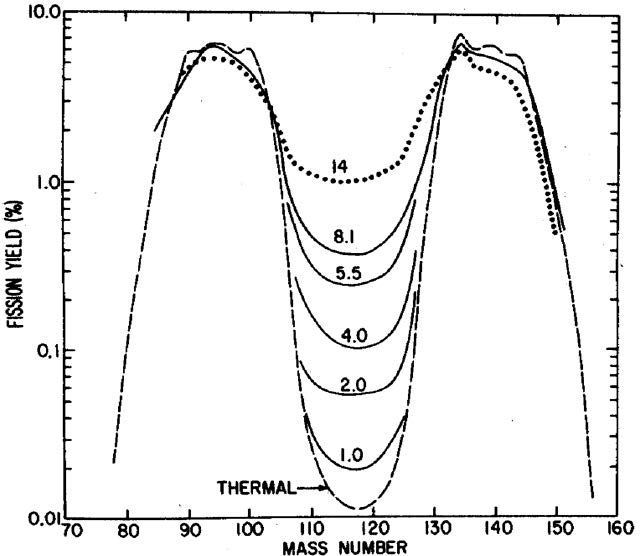
\includegraphics[scale=0.7]{../figs/FP_energy}
\caption{Fission product distribution from U-238 as a function of energy (MeV)}
\label{fig:fp-e}
\end{figure}
\begin{figure}
\centering
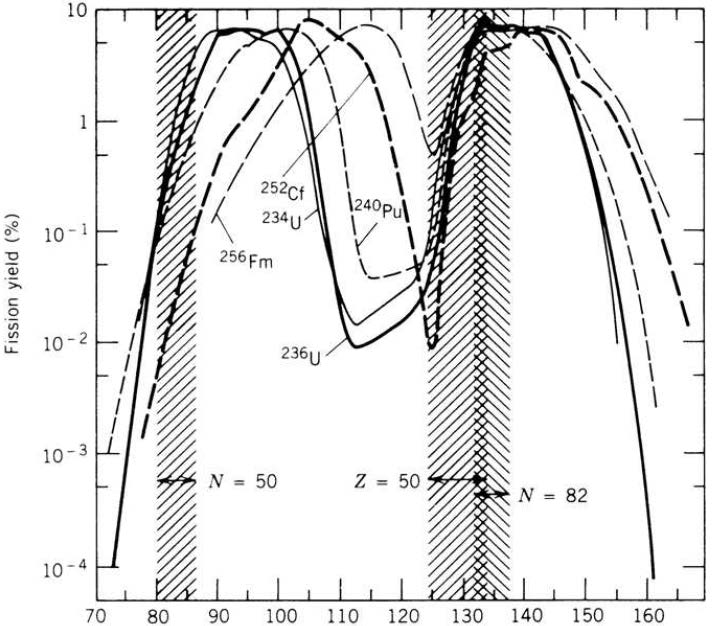
\includegraphics[scale=0.7]{../figs/FP_Isotope}
\caption{Fission product distribution from different isotopes}
\label{fig:fp-i}
\end{figure}


Most fission is asymmetric, with one fission product more massive than the other. In general the higher the energy of the state that undergoes nuclear fission, the more likely that the two fission products have similar mass. Hence as the neutron energy increases and/or the energy of the fissile atom increases, the valley between the two peaks becomes more shallow.

$\nu=$average number of neutrons per fission. See \autoref{fig:nu} for examples, where $\nu^{49}$ is for $^{239}$Pu, $\nu^{25}$ is for $^{235}$U, $\nu^{23}$ is for $^{233}$U.
\begin{center}
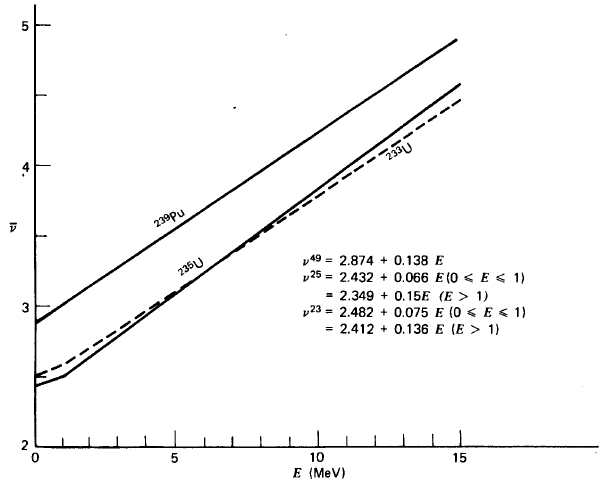
\includegraphics[scale=0.6]{../figs/nu}
\caption{average \# of neutrons release per fission as a function of energy}
\label{fig:nu}
\end{center}

$\alpha = \frac{\sigma_\gamma}{\sigma_f}$ is the capture-to-fission ratio

$\eta = \frac{\nu \sigma_f}{\sigma_a}$ is the average number of neutrons produced per neutron absorbed. For a single fissile isotope we can write $\eta = \frac{\nu}{1+\alpha}$

conversion ratio = $\frac{\text{fissile produced}}{\text{fissile consumed}}$

In thermal reactors, the conversion ratio is typically less than one. In fast reactors, the conversion ratio can be greater than or equal to one. This is the motivation for ``breeding" reactors and requires $\eta >2$.

\begin{center}
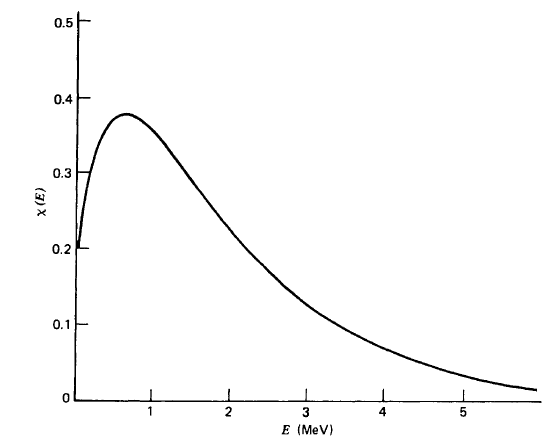
\includegraphics[scale=0.6]{../figs/fissionspectrum}
\end{center}
$\chi(E)dE=$ fission spectrum = probability that a neutron will have energy\\ $E$ in the range $[E, E+dE]$

The prompt neutron fission spectrum of $^{235}$U: $\chi(E) = 0.453 e^{-1.036E}\sinh\sqrt{2.29E}$

Fission produces both prompt and delayed neutrons, where the delayed neutrons come from the decay of various unstable fission products. We define: $\beta=\frac{\nu_{delayed}}{\nu_{total}}$. Delayed neutrons are usually split into six groups, based on the half-lifes of the unstable fission products.

The majority of the energy released in a fission event is in form of the kinetic energy of the fission products. For $^{235}$U fission:

KE of FP $\approx 168$ MeV

KE of $n\approx 5$ MeV

prompt $\gamma$ $E\approx 7$ MeV

$\beta^- E$ from FP decay $\approx 8$ MeV

$\gamma E$ from FP decay $\approx 7$ MeV

neutrino $E$ from FP decay $\approx 12$ MeV

All of the kinetic energy from the fission products and neutrons is considered recoverable. Most of the $\gamma$ energy and all of the $\beta^-$ energy is recoverable. None of the neutrino energy is recoverable. In total, $~207$ MeV is emitted and $~195$MeV is recoverable.

\section*{Multiplication Factor and Nuclear Criticality}

$k=\frac{\text{\# of neutrons produced}}{\text{\# of neutrons lost}}$ (multiplication factor)

$p=$ resonance escape probability = fraction of fission neutrons that manage to slow down from fission to thermal energies without being absorbed.

$f=$ thermal utilization factor = conditional probability that if neutron is absorbed, it will be absorbed in the fuel.

$\epsilon=$ fast fission factor = total number of fission neutrons / number of fission neutrons from thermal fission.

The four-factor formula assumes an infinite homogeneous system with two neutron groups (fast + thermal):
\[
k_{\infty}=\epsilon p f \eta
\]

The six-factor formula accounts for fast and thermal neutron leakage in finite systems:
\[
k_{eff} = P_{FNL}P_{TNL}\epsilon p f\eta
\]

\section*{Neutron Transport}

At any time $t$ we use six variables to specify the
position of any particle in phase space: three position variables denoted by the vector $\rvec$,
the kinetic energy $E$, and a unit vector $\omvec$, which indicates the direction in which the
particle is traveling. With these variables we can define the distribution function
$N(\rvec,E,\omvec,t)$,
such that
\begin{align*}
N(\rvec,E,\omvec,t)dVdEd\omvec = \begin{array}{l}
\text{the number of particles in a differential volume}\vspace{-0.1 cm}\\
\text{element $dV$ at spatial point $\rvec$, with energy in $dE$}\vspace{-0.1 cm}\\
\text{about $E$, traveling in a solid angle element $d\omvec$}\vspace{-0.1 cm}\\
\text{about $\omvec$, at time $t$.}
\end{array}\label{nmbpart}
\end{align*} 

 Let the vector $\rvec$ be described by the Cartesian coordinates $x$, $y$, $z$, and the vector
$\omvec$ be described by a polar angle $\theta$ measured with respect to the $z$-axis
 and a corresponding azimuthal angle $\varphi$ such that $(\Omega_x=\cos\varphi \sin\theta, \Omega_y = \sin\varphi \sin\theta, \Omega_z = \cos\theta)$.
\begin{figure}%[t]\nonumber
\includegraphics[height=10 cm,width=10 cm]{../figs/fig2_1.jpg}
\end{figure}
 If we introduce $\mu = \cos\theta$, then
\begin{align*}
dV &= dxdydz\,,
\\
d\omvec &=  \sin\theta d\theta d\varphi = d\mu d\varphi\,. 
\end{align*}
A minus sign was omitted since $\mu$ runs from
1 to -1 when $\theta$ runs from 0 to $\pi$.
If $\vec{v}$ is the velocity vector, then $\omvec = \vec{v}/{|\vec{v}|}$,
and
it is easy to see that the components of the particle's velocity in the Cartesian
coordinates are given by
\begin{align*}
\dot x &=  v\Omega_x\,,\\
\dot y &=  v\Omega_y\,,\\
\dot z &=  v\Omega_z\,,
\end{align*}
 where $v$ is the particle's speed in the nonrelativistic case; that is, $v = \sqrt{2E/m_p}$, with $m_p$
denoting the particle's mass.

\subsection*{Integral approach to the transport equation}

Angular neutron flux:
\[
\varphi(\rvec, E, \omvec, t)=vN(\rvec, E, \omvec, t).
\] 

[Note: in order not to confuse the angular flux $\varphi$ with the azimuthal angle, we will write the azimuthal angle as $\overline{\varphi}$. In these notes the notation $\varphi$ for the angular flux was used to be consistent with the text book; in most references the angular flux is written as $\psi$.]

Consider a well-defined control volume $V$ and assume that $N(\rvec, E, \omvec, t)$ is known. How many neutrons are in $V$ with energy $E$ and direction $\omvec$?

$\left[\int_V dV N(\rvec, E, \omvec, t)\right] dEd\omvec =$ \# of neutrons in $V$ with energy $E$ and direction $\omvec$

$\frac{\partial}{\partial t}\left[\int_V dV N(\rvec, E, \omvec, t)\right] dEd\omvec =$ rate of change  = gain rate - loss rate

Neutron gains come from a source (fission) or in-scattering $(E', \omvec' \rightarrow E, \omvec)$. Neutron losses come from collisions $(E, \omvec \rightarrow E', \omvec')$ and streaming.

$\left[\int_V dV S(\rvec, E, \omvec, t)\right] dEd\omvec =$ internal source of neutrons.

The double differential in-scattering cross section is expressed as $\Sigma_s(E'\rightarrow E, \omvec'\rightarrow\omvec)$.

The entire scattering term is
$\left[\int_VdV\int_0^{\infty}dE'\int_{4\pi}d\omvec'\Sigma_s(E'\rightarrow E,\omvec'\rightarrow\omvec)\varphi(\rvec,E',\omvec',t)\right]dEd\Omega$

The collision term is
$\left[\int_VdV\Sigma_{t}(\rvec,E)\varphi(\rvec,E,\omvec,t)\right]dEd\Omega$

The streaming term is
$\left[\int_VdV div \vec{j}(\rvec, E, \omvec,t)\right]dEd\Omega$ where $\vec{j}(\rvec,E,\omvec,t)=\varphi(\rvec,E,\omvec,t)\omvec$

Finally:
\begin{align*}
&\frac{\partial}{\partial t}\left[\int_V dV N(\rvec, E, \omvec, t)\right] dEd\omvec =
\left[\int_V dV S(\rvec, E, \omvec, t)\right] dEd\omvec +
\\& \hspace{1cm} \left[\int_VdV\int_0^{\infty}dE'\int_{4\pi}d\omvec'\Sigma_s(E'\rightarrow E,\omvec'\rightarrow\omvec)\varphi(\rvec,E',\omvec',t)\right]dEd\Omega \,-
\\& \hspace{2cm}\left[\int_VdV\Sigma_{t}(\rvec,E)\varphi(\rvec,E,\omvec,t)\right]dEd\Omega - \left[\int_VdV div \vec{j}(\rvec, E, \omvec,t)\right]dEd\Omega
\end{align*}

\begin{align*}
\frac{1}{v}\frac{\partial}{\partial t}\varphi(\rvec, E, \omvec, t) &=
 S(\rvec, E, \omvec, t) +
 \int_0^{\infty}dE'\int_{4\pi}d\omvec'\Sigma_s(E'\rightarrow E,\omvec'\rightarrow\omvec)\varphi(\rvec,E',\omvec',t) \,-
\\& \hspace{1cm}\Sigma_{t}(\rvec,E)\varphi(\rvec,E,\omvec,t) - div \vec{j}(\rvec, E, \omvec,t)
\end{align*}

Initial condition:
\[
\varphi(\rvec, E, \omvec, 0) = \varphi_0(\rvec, E,\omvec)
\]

Void boundary condition:
\[
\varphi(\rvec_s, E, \omvec, t) = 0, \,\,\, \rvec_s \, \in \, \partial V \,\,\, \text{and} \,\,\, \omvec \cdot \vec{n} <0.
\]

\subsection*{Another approach to the transport equation}


We consider a six-dimensional volume (as a six-dimensional cube)
 fixed in space, of dimensions
$\triangle x$, $\triangle y$, $\triangle z$, $\triangle E$, $\triangle \mu$, $\triangle \overline\varphi$.
Then, the number of particles within this volume at time $t$ is
\begin{equation*}
N(\rvec,E,\omvec,t)\triangle x\triangle y\triangle z\triangle E\triangle \mu\triangle \overline\varphi =
N(\rvec,E,\omvec,t)\triangle \beta,
\end{equation*}
where all arguments of $N$ are ``average" arguments in the %volume $\triangle V$.
increment of six-dimensional phase space $\triangle \beta$.
The number of
particles in this cube changes with time:
\begin{equation*}
\triangle \beta\frac{\partial}{\partial t}N(\rvec,E,\omvec,t) = \begin{array}{l}
\text{time rate of change of the number of}\vspace{-0.1cm}\\
\text{particles in the six-dimensional cube $\triangle \beta$.}
\end{array}
\end{equation*}
 This time rate of change is due to five separate processes. One is the rate of streaming of
particles out of the volume through the boundaries. The others occur within the
six-dimensional ``cube": the rate
of absorption; the rate of scattering from $E$, $\omvec$ to all other energies and directions, known
as outscattering; the rate of scattering into $E$, $\omvec$ from all other energies and
 directions, known as inscattering; and the rate of production of particles due to an internal source.

 Now, let us consider the surfaces of the cube perpendicular to the $x$-axis. For the net rate
of particles leaving the cube through these two surfaces, we have
\begin{equation*}
(\textrm{Streaming})_x = \dot x N(\rvec,E,\omvec,t)\mid_x^{x+\triangle x}
\triangle y\triangle z\triangle E\triangle \mu\triangle \overline\varphi,
\end{equation*}
 where $\dot x$ is the $x$ component of the particle velocity,
and 
$\triangle y\triangle z\triangle E\triangle\mu\triangle \overline\varphi$ is the surface area. Letting $\triangle x$ go to
the differential $dx$, we rewrite
\begin{equation*}
(\textrm{Streaming})_x = \triangle \beta \frac{\partial}{\partial x}\big[
\dot x N(\rvec,E,\omvec,t)\big].
\end{equation*}
 Using the same procedure for the flow from the cube in the other five ``directions", we obtain
\begin{align*}
\textrm{Streaming} =
\bigg[ \frac{\partial}{\partial x}(\dot x N) + &
\frac{\partial}{\partial y}(\dot y N) +\frac{\partial}{\partial z}(\dot z N) \\
&\quad\quad + \frac{\partial}{\partial E}(\dot E N) + \frac{\partial}{\partial \mu}(\dot \mu N) +
\frac{\partial}{\partial \overline{\varphi}}(\dot \varphi N)\bigg] \triangle \beta,
\end{align*}
 where $N = N(\rvec,E,\omvec,t)$.


 The rate of absorption within the cube is the product of the number of particles in the cube
and the probability of absorption per particle per unit of time. This probability is given by
the product of the absorption cross section and the particle speed $v$. That is,
\begin{equation*}
\textrm{Absorption} = v\Sigma_a(\rvec,E)N(\rvec ,E,\omvec,t)\triangle \beta.
\end{equation*}
 Using similar arguments and the fact that we need to sum the scattering from (to) $E$,
$\omvec$ to (from) all other energies and directions $E'$, $\omvec'$, we find
\begin{align*}
\textrm{Outscattering} &= \triangle \beta \int_0^{\infty}\int_{4\pi}
v\Sigma_s(\rvec,E\rightarrow E', \omvec\rightarrow\omvec')N(\rvec,E,\omvec,t)d\omvec'dE', \\
\textrm{Inscattering} &= \triangle \beta \int_0^{\infty}\int_{4\pi}
v'\Sigma_s(\rvec,E'\rightarrow E, \omvec'\rightarrow\omvec,)N(\rvec,E',\omvec',t)d\omvec'dE',
\end{align*}
 where $\Sigma_s(\rvec,E'\rightarrow E, \omvec'\rightarrow\omvec)$ is the macroscopic differential scattering cross section. Since the distribution function in the integrand of the outscattering term is independent of
 the integration variables, we can rewrite
Outscattering as $\triangle \beta v\Sigma_s(\rvec,E)N(\rvec, E, \omvec,t).$
Finally, we need to consider the internal source of particles. We
quantify this source  by introducing the function $S(\rvec, E, \omvec, t)$
such that the rate of introduction of particles into the cube is given by
\begin{equation*}
\textrm{Source} = S(\rvec,E,\omvec,t)\triangle \beta.
\end{equation*}

 In order to build the transport equation, we sum these equations with appropriate signs
for loss and gain, to the overall rate of change. Letting $\triangle \beta$ approach a differential
element and canceling it, we obtain
\begin{align}
\frac{\partial N}{\partial t} =& -\left[\frac{\partial (\dot x N)}{\partial x} +
\frac{\partial (\dot y N)}{\partial y}+\frac{\partial (\dot z N)}{\partial z} +
\frac{\partial (\dot E N)}{\partial E}+\frac{\partial (\dot \mu N)}{\partial \mu}+
\frac{\partial (\dot \varphi N)}{\partial \overline\varphi}\right] 
\\ & \quad - v\Sigma_a(\rvec,E)N \nonumber
 \\& \quad\quad\quad   + 
\int_0^{\infty}\int_{4\pi}v'\Sigma_s(\rvec, E'\rightarrow E,\omvec'\rightarrow\omvec)N(\rvec,E',\omvec',t) d\omvec'dE'\nonumber 
\\& \quad\quad\quad\quad\quad\quad -\int_0^{\infty}\int_{4\pi}v\Sigma_s(\rvec, E\rightarrow E',\omvec\rightarrow\omvec')N(\rvec,E,\omvec,t) d\omvec'dE'\nonumber
\\& \quad\quad\quad\quad\quad\quad\quad\quad\quad
+S(\rvec,E,\omvec,t),\nonumber
\end{align}
 where $N = N(\rvec,E,\omvec,t)$. Since particles travel in a straight line
between collisions, \linebreak
$\dot \mu = \dot \varphi = 0$. Furthermore, $\dot E = 0$ because particles stream
with no change in energy. Finally, performing the outscattering integral:
\begin{align}
&\frac{1}{v}\frac{\partial \varphi}{\partial t}(\rvec,E,\omvec,t) + \omvec\cdot  \nabla \varphi(\rvec,E,\omvec,t) +
 \Sigma_t(\rvec,E)\varphi(\rvec,E,\omvec,t)
\\& \quad =
\int_0^{\infty}\int_{4\pi}\Sigma_s(\rvec, E'\rightarrow E,\omvec'\rightarrow\omvec)
\varphi(\rvec,E',\omvec',t)d\omvec'dE'+S(\rvec, E, \omvec,t) \nonumber.
\end{align}

We can easily generalize this equation to include nuclear fission.
To do that, we must revisit our treatment of $\Sigma_a$; as we have mentioned, there are two main processes responsible for the absorption of particles in the system: \textit{radiative capture} and \textit{nuclear fission}. Now, we define
\begin{align*}
\Sigma_\gamma(\rvec,E)ds = \textrm{probability of capture}
\end{align*}
and
\begin{align*}
\Sigma_f(\rvec,E)ds = \textrm{probability of a fission event},
\end{align*}
such that
\begin{align*}
\Sigma_a(\rvec,E) = \Sigma_\gamma(\rvec,E) + \Sigma_f(\rvec,E)\,.
\end{align*}

While a captured neutron is simply removed from the system, a neutron with energy $E$ that induces a fission event causes the target nucleus to split into two smaller daughter nuclei, and 
\begin{align*}
\nu(E) = \textrm{the mean number of fission neutrons that are released}\,.
\end{align*}
Of this number, $\nu(E)[1-M(E)]$ are \textit{prompt} fission neutrons (being emitted within $10^{-15}$ seconds of the fission event). These fission neutrons are emitted isotropically, with an energy distribution given by the fission spectrum $\chi_p(E)$. Also, $\nu(E)M(E)$ \textit{delayed} fission neutrons (being released roughly 0.1 to 60 seconds after the fission event) are created; a delayed neutron is produced when a radioactive daughter nucleus undergoes a radioactive decay process in which a neutron is emitted. 

Assuming (for simplicity) that the number of delayed neutrons emitted by fission is very small [$M(E)<<1$], we can neglect the delayed neutron terms and rewrite
the transport equation as
\begin{align}
&\frac{1}{v}\frac{\partial \varphi}{\partial t}(\rvec,E,\omvec,t) + \omvec\cdot  \nabla \varphi(\rvec,E,\omvec,t) +
 \Sigma_t(\rvec,E)\varphi(\rvec,E,\omvec,t) 
\\& \quad\quad\quad\quad =
\int_0^{\infty}\int_{4\pi}\Sigma_s(\rvec, E'\rightarrow E,\omvec'\rightarrow\omvec)
\varphi(\rvec,E',\omvec',t)d\omvec'dE'\nonumber
\\&\quad\quad\quad\quad\quad\quad +\frac{\chi_p(E)}{4\pi}\int_0^{\infty}\int_{4\pi}\nu(E')\Sigma_f(\rvec,E')
\varphi(\rvec,E',\omvec',t)d\omvec'dE'\nonumber
\\&\quad\quad\quad\quad\quad\quad\quad\quad+S(\rvec, E, \omvec,t) \nonumber.
\end{align}
   
These equations require both spatial and temporal boundary conditions.
Assuming that the
physical
system of interest is nonreentrant (convex) and characterized by a
volume $V$, it is sufficient to specify the flux of
particles at all points of the bounding surface of the system in the incoming
directions. This implies
\begin{align*}
\varphi(\rvec_s, E,\omvec,t) &= \varphi_b(\rvec_s,E,\omvec,t)\,, \hspace{0.5 cm} \textbf{n} \cdot \omvec <0,
\end{align*}
 where $\varphi_b$ is a specified function at the boundary, $\rvec_s$ is a point on the surface, and $\textbf{n}$ is the unit
outward normal vector at this point. In the time variable, we assume the range of
interest $0\leq t<\infty$ and specify the
initial condition at $t=0$, such that
\begin{align*}
\varphi(\rvec,E,\omvec,0) = \varphi_0(\rvec,E,\omvec),
\end{align*}
 where $\varphi_0$ is a specified function.
 
It is common to make extra assumptions in order to obtain a simpler version of these equations. For instance, in the case of time-independent, monoenergetic particle transport in a homogeneous medium with a known interior isotropic source:
\begin{align*}
\omvec\cdot  \nabla \varphi(\rvec,\omvec) +
 \Sigma_t\varphi(\rvec,\omvec)
=
\int_{4\pi}\Sigma_s(\omvec'\rightarrow\omvec)
\varphi(\rvec,\omvec')d\omvec'+\frac{S(\rvec)}{4\pi}\,,
\end{align*}
and 
\begin{align*}
\omvec\cdot  \nabla \varphi(\rvec,\omvec) +
 \Sigma_t\varphi(\rvec,\omvec)%\\&
 &=
\int_{4\pi}\Sigma_s(\omvec'\rightarrow\omvec)
\varphi(\rvec,\omvec')d\omvec'\\&\quad\quad\quad\quad\quad\quad
 +\frac{\nu\Sigma_f}{4\pi}\int_{4\pi}
\varphi(\rvec,\omvec')d\omvec'+\frac{S(\rvec)}{4\pi}\,.\nonumber
\end{align*}
Both the equations above need a spatial boundary condition, which is given by
\begin{align*}
\varphi(\rvec_s,\omvec) = \varphi_b(\rvec_s,\omvec)\,, \hspace{0.5 cm} \textbf{n} \cdot \omvec <0\,.
\end{align*}

In steady-state reactor calculations, one often sees a version of these equations in which the inhomogeneous source $S(\rvec)$ and the boundary source $\varphi_b(\rvec_s,\omvec)$ are set to zero, and the fission source is modified by a constant factor $1/k$:
\begin{align*}
&\omvec\cdot  \nabla \varphi(\rvec,\omvec) +
 \Sigma_t\varphi(\rvec,\omvec)%\\&
 =
\int_{4\pi}\Sigma_s(\omvec'\rightarrow\omvec)
\varphi(\rvec,\omvec')d\omvec'\\&\quad\quad\quad\quad\quad\quad\quad\quad\quad\quad\quad\quad\quad\quad\quad\quad\quad\quad
 +\frac{\nu\Sigma_f}{4\pi k}\int_{4\pi}
\varphi(\rvec,\omvec')d\omvec'\,,\nonumber\\
&\varphi(\rvec_s,\omvec) = 0, \hspace{0.5 cm} \textbf{n} \cdot \omvec <0\,.
\end{align*}
These equations always have the zero solution $\varphi = 0$; the goal is to find the largest value of $k$ such that a nonzero solution $\varphi$ exists. The resulting $k$ is called the \textit{criticality} (or \textit{criticality eigenvalue}) of the system. If a system has a fissile region, it can be shown that $k$ always exists, and the corresponding (eigenfunction) $\varphi$ is unique and positive.


\end{document}
